\documentclass[x11names]{article}
\usepackage[a4paper, total={6in, 9in}]{geometry}
\usepackage[skins]{tcolorbox}
\usepackage{tikz}
\usetikzlibrary{arrows}
\usetikzlibrary{calc}
\usepackage{pgfplots}
\pgfplotsset{compat=1.9}
\usepgflibrary{shapes.geometric}
\usepackage{xcolor}
\usepackage{amsmath}
%\usepackage{fourier-oft}
\usepackage{mathrsfs}
\usepackage{amssymb}
\usepackage{hyperref}
\usepackage{enumitem}
%% custom
\renewcommand*\contentsname{Indice}
\setcounter{tocdepth}{4}
\setcounter{secnumdepth}{2}
\pgfplotsset{compat=1.15}

% boxes
\definecolor{myblue}{RGB}{224, 245, 255} 
\definecolor{myred}{RGB}{198, 247, 211}
\definecolor{myorange}{RGB}{255, 102, 0}

\newtcolorbox{es}[2][]{%
	enhanced,
	sharp corners, % Angoli netti
	boxrule=0.4pt, % Spessore del bordo
	colback=white, % Colore di sfondo
	colframe=black, % Colore del bordo
	coltitle=black, % Colore del titolo
	fonttitle=\itshape, % Font del titolo in corsivo
	attach boxed title to top left={yshift=-0.5\baselineskip-0.4pt,xshift=2mm},
	boxed title style={tile, size=minimal, left=0.5mm, right=0.5mm,
		colback=white, before upper=\strut, boxrule=0.5pt, colframe=black},
	title=#2, % Testo del titolo
	borderline east={0.4pt}{0pt}{black,dashed}, % Bordo tratteggiato a est
	borderline west={0.4pt}{0pt}{black,dashed}, % Bordo tratteggiato a ovest
	borderline south={0.4pt}{0pt}{black,dashed}, % Bordo tratteggiato a sud
	borderline north={0.4pt}{0pt}{black,dashed}, % Bordo tratteggiato a nord
	#1 % Parametro opzionale aggiuntivo
}
\newtcolorbox{dym}[2][]{%
	enhanced,colback=white,colframe=black,coltitle=black,
	sharp corners,boxrule=0.4pt,
	fonttitle=\itshape,,
	attach boxed title to top left={yshift=-0.5\baselineskip-0.4pt,xshift=2mm},
	boxed title style={tile,size=minimal,left=0.5mm,right=0.5mm,
		colback=white,before upper=\strut},
	title=#2,#1
}
\newtcolorbox{blues}[2][]{%
	enhanced,colback=myblue,colframe=black,coltitle=black,
	sharp corners,boxrule=0.4pt,
	fonttitle=\bfseries\itshape,
	attach boxed title to top left={yshift=-0.5\baselineskip-0.4pt,xshift=2mm},
	boxed title style={tile,size=minimal,left=0.5mm,right=0.5mm,
		colback=myblue,before upper=\strut},
	title=#2,#1
}
\newtcolorbox{redes}[2][]{%
	enhanced,colback=myred,colframe=black,coltitle=black,
	sharp corners,boxrule=0.4pt,
	fonttitle=\bfseries\itshape,
	attach boxed title to top left={yshift=-0.5\baselineskip-0.4pt,xshift=2mm},
	boxed title style={tile,size=minimal,left=0.5mm,right=0.5mm,
		colback=myred,before upper=\strut},
	title=#2,#1
}


\newcommand*{\QEDA}{\null\nobreak\hfill\ensuremath{\blacksquare}}%
\newcommand*{\QEDB}{\null\nobreak\hfill\ensuremath{\square}}%

\newcommand{\esempio}[2]{
	\begin{es}{esempio #1}
		#2
	\end{es}
}
\newcommand{\definizione}[2]{
	\begin{center}
		\fboxsep11pt
		\colorbox{myblue}{\begin{minipage}{5.75in}
				\begin{blues}{Definizione: #1}
					#2
				\end{blues}
		\end{minipage}}
	\end{center}
}
\newcommand{\teorema}[2]{
	\begin{center}
		\fboxsep11pt
		\colorbox{myred}{\begin{minipage}{5.75in}
				\begin{redes}{#1}
					#2
				\end{redes}
		\end{minipage}}
	\end{center}
}
\newcommand{\dimostrazione}[2]{
	\begin{dym}{dimostrazione: #1}
		#2
		\QEDB
	\end{dym}
}

\pgfplotsset{my axis/.append style={height=9cm,width=9cm,grid=major,samples=100,yticklabel=\empty,xticklabel=\empty}}
\pgfplotsset{my plot/.append style={thick,samples=500}}

\begin{document}
	
\begin{titlepage}
	\begin{center}
		\vspace*{1cm}
		
		\textbf{\LARGE Relazione di laboratorio - Pendolo semplice}
		
		\vspace{0.3cm}
		\large \textit{Misura del periodo di un pendolo semplice} \\
		
		\vspace{0.5cm}
		\Large Federico Cesari \\
		
		\small 1096759 
		\vspace{0.2cm}
		
		\small Gruppo 5
		
		
		\vspace{3cm}
		\begin{center}
			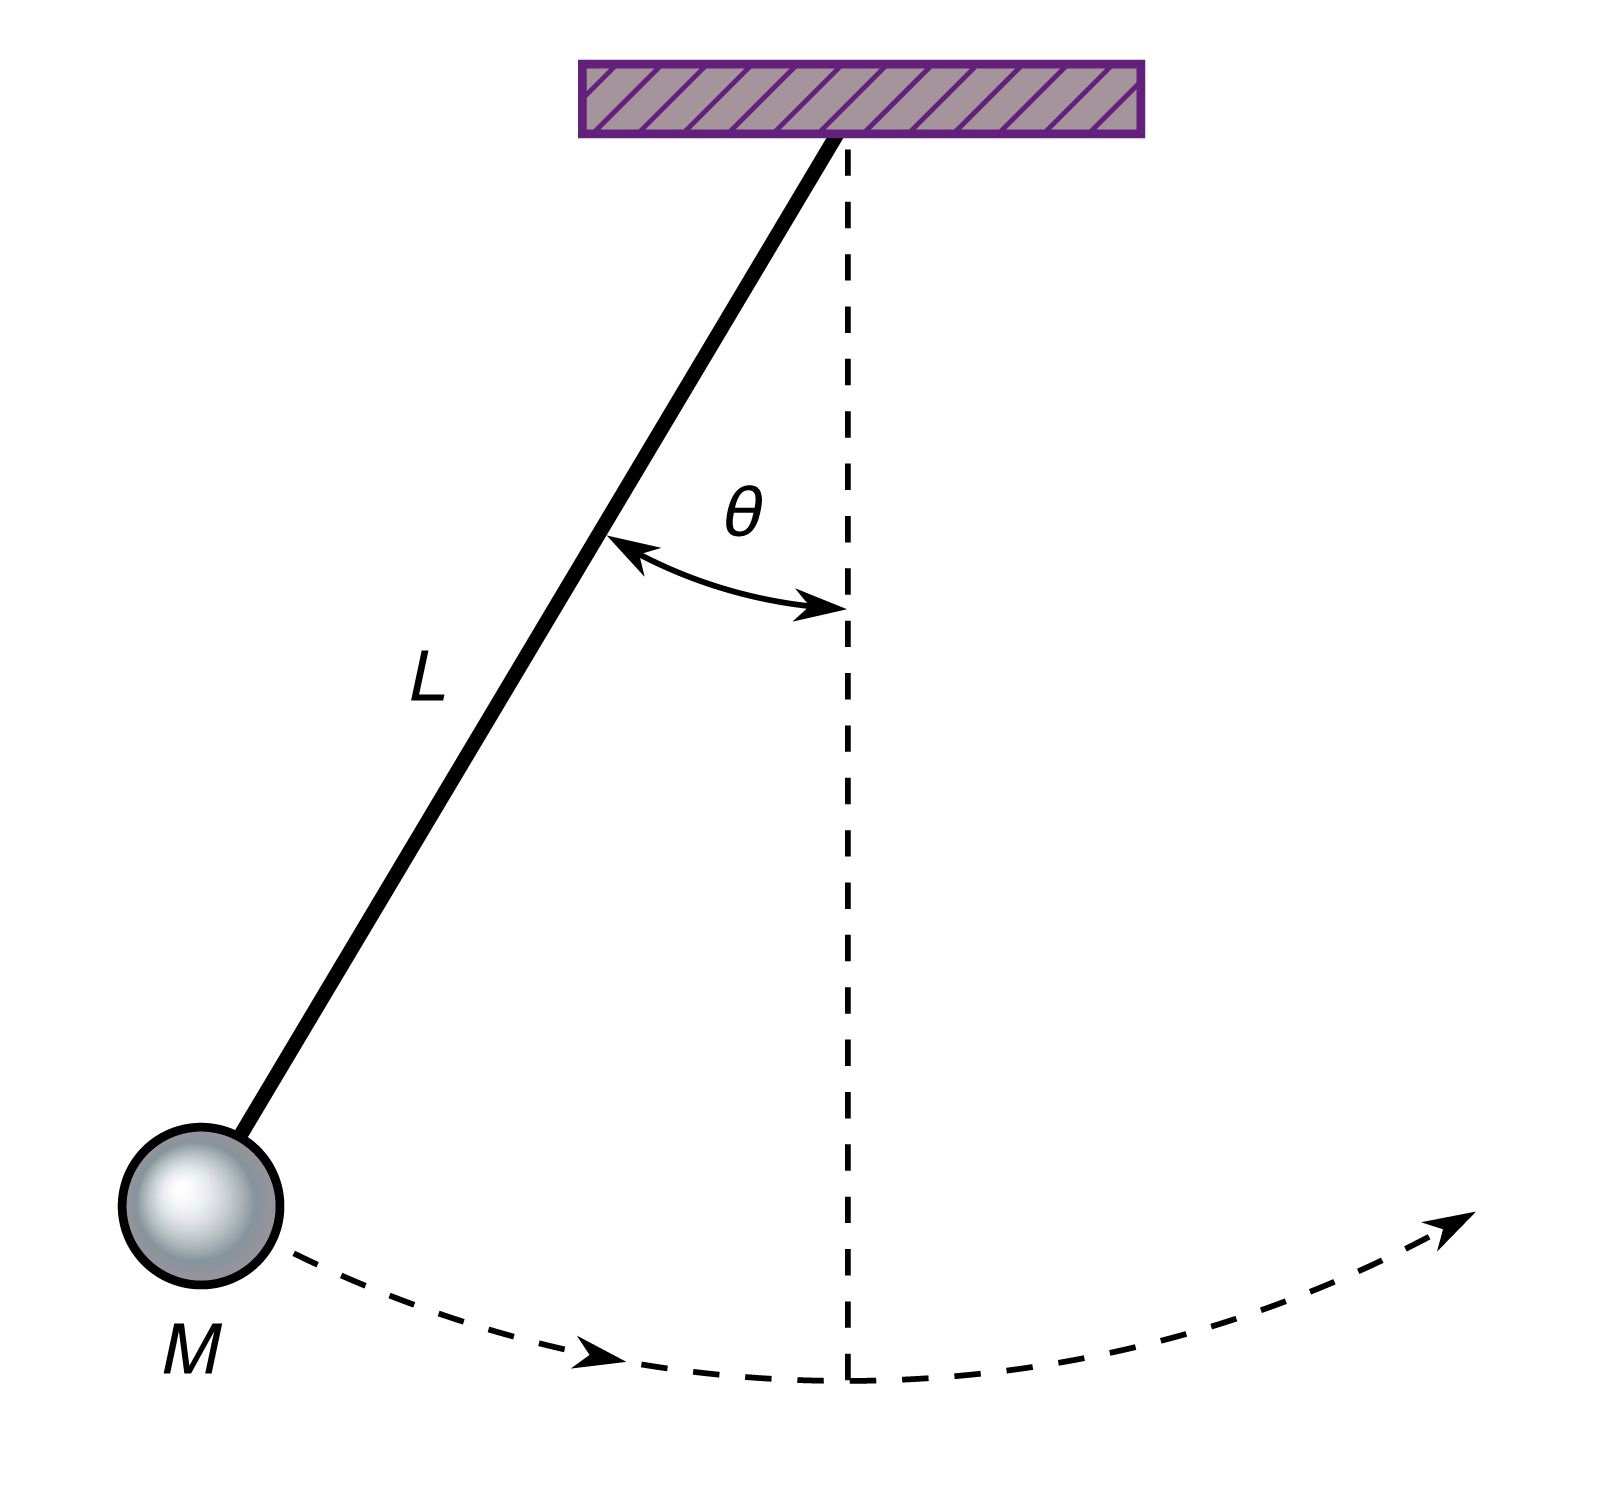
\includegraphics[scale=0.1]{IMG_0200.jpeg}	
		\end{center}
		
		
		
		\vfill
		
		
		
		corso A\\
		Università degli studi di Torino, Torino\\
		4 aprile 2024\\
		
		
	\end{center}
\end{titlepage}
\tableofcontents
\newpage
	
	
\section{Successioni di funzioni}

%\begin{center}
%\begin{tikzpicture}
%	\begin{axis}[my axis,xmin=-1,xmax=1]
%		\addplot[my plot, domain y=-pi/2:pi/2] {atan(x)};
%		\addplot[my plot, domain y=-pi/2:pi/2] {atan(2*x)};
%		\addplot[my plot, domain y=-pi/2:pi/2] {atan(20*x)};
%	\end{axis}
%\end{tikzpicture}
%\end{center}

\[ 
A \subseteq \mathbb{R} \;\ (\text{o } \mathbb{C}), \;\ f_{n}: A \to \mathbb{R} \;\ (\text{o } \mathbb{C}), \;\ n \in \mathbb{N} 
\]
\[ 
\begin{array}{ccl}
	N & \to & \{\text{f.ni definite su } A\} \\
	n & \mapsto & f_{n}
\end{array}
\]
Vogliamo studiare come si comporta \((f_{n})_{n}\) quando \(n\to +\infty\).

\subsection{Limiti di successioni}


\definizione{Convergenza puntuale}
{Diciamo che la successione di funzioni \((f_{n})_{n}\), \(f_{n}:A\subseteq \mathbb{R}\to \mathbb{R}  (\text{o } \mathbb{C})\) \textbf{converge puntualmente} (o semplicemente) a una funzione  \(f\) sull'insieme \(E \subseteq A\) se 
\[ 
\forall x \in E, \;\ \lim_{n\to + \infty}f_{n}(x) = f(x)
\]
Notiamo che quest'ultimo limite è un limite di successione numerica, quindi
\[ 
\forall x \in E, \quad  \forall \varepsilon > 0 \;\ \exists \bar{n} = \bar{n}(\varepsilon,x) \;\ \text{t.c.} \;\ |f_{n}(x) - f(x)| < \varepsilon, \quad \forall n \geq \bar{n}
\]}

\definizione{Convergenza uniforme}{Diciamo che la successione di funzioni \((f_{n})_{n}\), \(f_{n}:A\to \mathbb{R}  \;\ (\text{o } \mathbb{C})\) \textbf{converge uniformemente} su \(E \subseteq A\) alla funzione \(f:E\to \mathbb{R}\) se
\[ 
\forall \varepsilon > 0 \quad \exists \bar{n} = \bar{n}(\varepsilon) \;\ \text{t.c.} \;\ |f_{n}(x) - f(x)| < \varepsilon \quad \forall n \geq \bar{n}
\]
equivalentemente
\[ 
\forall \varepsilon > 0 \quad \exists \bar{n} = \bar{n}(\varepsilon) \;\ \text{t.c.} \;\ \text{sup}|f_{n}(x) - f(x)| < \varepsilon \quad \forall n \geq \bar{n}
\]
dove l'estremo superiore viene denominato \(\alpha_n\) successione positiva (\(\geq 0\)):
\[ 
\forall \varepsilon > 0 \quad \exists \bar{n} = \bar{n}(\varepsilon) \;\ \text{t.c.} \;\ 0 \leq \alpha_n < \varepsilon \quad \forall n \geq \bar{n}
\]
opure
\[ 
\
\]
} 


\esempio{1}{SKJFSjkajdfdajf  jf adksòl jfd jsaf
adf kjajsò fjkda òsf òdsa jf j

fjalkdòjf kjdskfjkdsajfk jads jfd fkdsfjkjdakfj kjd fdjfkjdsfò afdjòasdjf  ds

fjkad jfajdskòl jfòas jf jfkjò fjaò jfaò}
\esempio{2}{}
\esempio{3}{}



\teorema{Teorema 1 - La convergenza unifore preserva la continuità}{
Sia \((f_{n})_{n}\) una successione di funzioni \(f_{n}:A\subseteq \mathbb{R}\to \mathbb{R} \;\ (\text{o } \mathbb{C})\) tali che
\begin{enumerate}[start=1,label={(\itshape H\arabic*)}]
	\item \(f_{n}\) sono funzioni continue su \(E\subseteq A\),
	\item \(f_{n}\) converge uniformemente a \(f\) su \(E\)
\end{enumerate}
allora \(f\) è continua su \(E\)
}
\dimostrazione{}{
La tesi è 
\[ 
\forall x_{0} \in E, \;\ \lim_{x\to x_{0}} f(x) = f(x_{0})
\]
ovvero che
\[ 
\forall x_{0} \in E \qquad \forall \varepsilon > 0 \;\ \exists \delta = \delta(x_{0},\varepsilon) \;\ \text{t.c.} \;\ |f(x) - f(x_{0})| < \varepsilon \qquad \forall x \in (x_{0}-\delta,x_{0}+\delta) \cap E 
\]
\begin{itemize}
	\item Da (\textit{H2}) sappiamo che \( \lim_{n\to + \infty} \alpha _{n}\) quindi 
	\[\exists \bar{n} = \bar{n}(\varepsilon) \;\ \text{tale che} \;\ \alpha_{n} < \frac{\varepsilon}{3} \quad \forall n\geq\bar{n}
	\]
	\item Da (\textit{H1}) abbiamo invece la continuità di \(f_{n}\) in \(x_{0}\):
	\[ 
	\exists \delta = \delta(x_{0},\varepsilon) \;\ : \;\ | f_{n}(x) - f
	\]
\end{itemize}
\teorema{Teorema 2}{}
\dimostrazione{}{}

\esempio{4}{}

\teorema{Teorema}{}


% SERIE DI FUNZIONI
\section{Serie di funzioni}
Presa \((f_{n})_{n}\) successione di funzioni, \(f_{n}:A\subseteq \mathbb{R} \to \mathbb{R}\) (o \(\mathbb{C}\)), chiamiamo \textbf{serie di funzioni}, indicata con
\[ 
\sum_n f_{n}(x)
\]
la successione delle ridotte 
\[ 
S_{N} = \sum_{n=1}^N f_{n}(x)
\]
\paragraph{Convergenza della serie} Diciamo che la serie converge (puntualmente o uniformemente) su un insieme \(E\subseteq A\) se lo fa la successione delle ridotte. Si andrà quindi a studiare il limite di \(S_{N}\) che chiamiamo somma della serie.

\teorema{Teorema 1S}{
Data \(f:A\subseteq \mathbb{R} \to \mathbb{R}\), se
\begin{itemize}
	\item \(f_{n}\) continue su \(E\subseteq A\);
	\item \(\sum_n f_{n}\) converge uniformemente su \(E\subseteq A\) alla somma \(S(x)\)
\end{itemize}
Allora \(S(x)\) è continua su \(E\).}
\teorema{Teorema 2S}{
Data \(f:A\subseteq \mathbb{R} \to \mathbb{R}\) e \(E = [a,b]\subseteq \mathbb{R}\), se
\begin{itemize}
\item \(f_{n}\) continue su \(E\subseteq A\);
\item \(\sum_n f_{n}\) converge uniformemente su \(E\subseteq A\) alla somma \(S(x)\)
\end{itemize}
Allora
\[ 
\int_{a}^{b} \sum f_{n}(x)dx \quad  = \quad \sum \int_{a}^{b}  f_{n}(x)dx 
\]}

\definizione{}{
	\[ 
	I_{s} = \left\{x \;\:\;\ \text{la serie considerata} \sum f_{n}(x) \text{converge semplicemente} \right\}
	\]
	per la serie \(\sum x^n\) si ha che \(I_{s} = (-1,1)\)
	\[ 
	I_{a} = \left\{x \;\:\;\ \text{la serie considerata} \sum |f_{n}(x)| \text{converge semplicemente} \right\}
	\]
}

\teorema{Teorema: m-test o criterio di convergenza totale}{
Date 
\begin{itemize}
	\item \((f_{n})_{n}\) successione di funzioni su \(E\subseteq \mathbb{R}\) (o in \(\mathbb{C}\));
	\item \((m_{n})_{n} \subseteq \mathbb{R}\) successione di numeri reali positivi. 
\end{itemize}
tali che
\begin{enumerate}[start=1,label={(\itshape H\arabic*)}]
	\item \(|f_{n}(x)|\leq m_{n}\) \(\forall x \in E\), \(\forall n\);
	\item \(\sum m_{n}(x) < + \infty\).
\end{enumerate}
Allora la serie \(\sum f_{n}(x)\) converge assolutamente in ongi punto di \(E\) è uniformemente su \(E\) \(\implies\) la serie converge totalmente.}




	
\end{document}